\documentclass[11pt, a4paper]{article}

% ── Packages ──────────────────────────────────────────────────────────────────
\usepackage[margin=1.1in]{geometry}
\usepackage{amsmath, amssymb}
\usepackage{booktabs}
\usepackage{graphicx}
\usepackage{xcolor}
\usepackage{hyperref}
\usepackage{caption}
\usepackage{float}
\usepackage{microtype}
\usepackage{parskip}
\usepackage{enumitem}
\usepackage{array}
\usepackage{lmodern}
\usepackage[T1]{fontenc}
\usepackage{colortbl}

\hypersetup{colorlinks=true, linkcolor=black, citecolor=black, urlcolor=black}

% ── Title ─────────────────────────────────────────────────────────────────────
\title{
  \vspace{-1cm}
  \Large\textbf{RL Global Equity Allocator} \\[0.4em]
  \large PPO-Based Macro-Driven ETF Rotation
}
\author{Capital Fund Research}
\date{March 2026}

% ══════════════════════════════════════════════════════════════════════════════
\begin{document}
\maketitle
\thispagestyle{empty}

\begin{abstract}
A PPO reinforcement learning agent is trained to rotate across six global equity ETFs and cash using a ten-dimensional macro-momentum state. Trained on 2004--2013 only, the standalone model achieves \textbf{13.3\% annualised return} and \textbf{Sharpe 0.75} out-of-sample (2014--2025), matching SPY. A drawdown-differential hybrid overlay reduces maximum drawdown from $-$34.6\% to $-$30.0\% (Calmar 0.38 $\to$ 0.41) at a cost of 99\,bps. The hybrid integrates positively into a mean-variance portfolio alongside existing AMMA sector models.
\end{abstract}

\tableofcontents
\newpage

% ══════════════════════════════════════════════════════════════════════════════
\section{Universe and Data}

\subsection{Traded Assets}

\begin{center}
\begin{tabular}{lll}
\toprule
\textbf{Ticker} & \textbf{Description} & \textbf{Region} \\
\midrule
SPY-US  & SPDR S\&P 500 ETF         & US \\
EWJ-US  & iShares MSCI Japan ETF    & Developed Asia \\
INDA-US & iShares MSCI India ETF    & Emerging Asia \\
MCHI-US & iShares MSCI China ETF    & Emerging Asia \\
EZU-US  & iShares MSCI Eurozone ETF & Developed Europe \\
BIL-US  & SPDR 1--3 Month T-Bill    & Cash / Risk-free \\
\bottomrule
\end{tabular}
\end{center}

\subsection{Signal Tickers (not traded)}

BMOM momentum composites are computed for three signal tickers fed into the state vector:

\begin{center}
\begin{tabular}{ll}
\toprule
\textbf{Ticker} & \textbf{Role} \\
\midrule
TLT-US  & Long-duration bond momentum; risk-off regime signal \\
VIXY-US & Volatility momentum; equity fear gauge \\
IBIT-US & Bitcoin momentum; cross-asset liquidity signal \\
\bottomrule
\end{tabular}
\end{center}

\subsection{Macro Features}

Seven FRED series, each normalised with a 252-day rolling z-score: Fed balance sheet (WALCL), US M2, TLT price, VIX (via VIXY), yield slope (10Y$-$2Y), S\&P 500 EPS, and EPS growth (QoQ).

\subsection{Data Split}

\begin{center}
\begin{tabular}{lll}
\toprule
\textbf{Period} & \textbf{Dates} & \textbf{Days} \\
\midrule
Training        & 2 Jan 2004 -- 31 Dec 2013  & 2,608 \\
Out-of-Sample   & 1 Jan 2014 -- 10 Sep 2025  & 3,051 \\
\bottomrule
\end{tabular}
\end{center}

% ══════════════════════════════════════════════════════════════════════════════
\section{Model Design}

\subsection{State, Action, Reward}

The agent observes $s_t \in \mathbb{R}^{10}$: seven normalised macro features and three BMOM composites.

\[
  \text{BMOM}(t) = 0.15\,r_{20} + 0.35\,r_{60} + 0.35\,r_{120} + 0.15\,r_{240}
\]

Triangular weights peak at the 60--120-day horizon, which empirically carries the strongest momentum signal.

At each timestep the agent selects one action $a_t \in \{1,\ldots,6\}$, allocating 100\% to a single ETF.

The reward is a mean-variance objective:

\[
  r_t = \mu_t - \lambda \cdot w^\top \Sigma_{60}\, w, \qquad \lambda = 2.0
\]

where $\mu_t$ is the daily return of the selected asset, $w$ is the one-hot weight vector, and $\Sigma_{60}$ is the rolling 60-day covariance matrix. This penalises selection of currently volatile assets and incentivises Sharpe-maximising behaviour.

\subsection{Network Architecture}

Policy and value networks share the same backbone:

\[
\mathbb{R}^{10}
\xrightarrow{\;\text{Linear}(128)\;+\;\text{LayerNorm}\;+\;\text{ReLU}\;}
\xrightarrow{\;\text{Linear}(128)\;+\;\text{LayerNorm}\;+\;\text{ReLU}\;}
\text{Output}
\]

The policy head appends Softmax over 6 actions; the value head outputs scalar $V_\phi(s)$. LayerNorm handles the heterogeneous scales of the macro inputs.

% ══════════════════════════════════════════════════════════════════════════════
\section{Training}

\subsection{PPO Objective}

\[
\mathcal{L}^{\text{CLIP}}(\theta) = \mathbb{E}_t \Big[
  \min\!\Big(
    \rho_t\, \hat{A}_t,\;
    \operatorname{clip}(\rho_t,\, 1{-}\varepsilon,\, 1{+}\varepsilon)\, \hat{A}_t
  \Big)
\Big]
\]

An entropy bonus prevents policy collapse; GAE is used for advantage estimation.

\subsection{Hyperparameters}

\begin{center}
\begin{tabular}{ll}
\toprule
\textbf{Parameter} & \textbf{Value} \\
\midrule
Policy / Value learning rate  & $3{\times}10^{-4}$ / $1{\times}10^{-3}$ \\
Discount $\gamma$             & 0.95 \\
PPO clip $\varepsilon$        & 0.20 \\
Entropy coefficient           & 0.01 \\
Update frequency              & 252 steps (1 trading year) \\
Training episodes             & 50 \\
Covariance window             & 60 days \\
Risk aversion $\lambda$       & 2.0 \\
Production seed               & 999 \\
\bottomrule
\end{tabular}
\end{center}

\subsection{Seed Selection}

Ten seeds were screened using 20-episode training runs; seed 999 was retrained for the full 50 episodes.

\begin{center}
\begin{tabular}{lcc}
\toprule
\textbf{Seed} & \textbf{OOS Sharpe (screen)} & \textbf{Top 2022 Holding} \\
\midrule
\textbf{999}  & \textbf{0.727} & SPY-US \\
1             & 0.720          & SPY-US \\
0             & 0.717          & SPY-US \\
2024          & 0.637          & SPY-US \\
42            & 0.626          & INDA-US \\
123           & 0.480          & INDA-US \\
7             & 0.372          & EZU-US \\
256           & 0.328          & EWJ-US \\
99            & 0.224          & SPY-US \\
512           & 0.110          & MCHI-US \\
\bottomrule
\end{tabular}
\end{center}

Seeds converging to non-US equity in 2022 underperformed; seed 999 correctly held SPY through the rate hike cycle.

% ══════════════════════════════════════════════════════════════════════════════
\section{Macro Factor Rationale}

Each ETF links to a primary macro driver the agent can condition on:

\begin{itemize}[leftmargin=*, itemsep=0.2em]
  \item \textbf{SPY:} inversely related to TLT; rate regime drives US equity rotation.
  \item \textbf{EZU:} yield-curve sensitive; inversion compresses European bank margins.
  \item \textbf{INDA:} co-moves with Fed balance sheet expansion; EM assets benefit from dollar liquidity.
  \item \textbf{MCHI:} tracks global M2 growth; leveraged play on nominal liquidity.
  \item \textbf{EWJ:} responds to yield-slope steepening; decouples from DM equities during US rate transitions.
  \item \textbf{BIL:} refuge when all risky assets exhibit elevated $w^\top \Sigma_{60} w$.
\end{itemize}

% ══════════════════════════════════════════════════════════════════════════════
\section{Hybrid Drawdown-Differential Overlay}

The standalone agent's concentrated one-hot allocation produces a $-$34.6\% max drawdown. The hybrid overlay provides a tail-risk floor without materially reducing returns.

\textbf{Mechanism.} Define the rolling drawdown differential $\Delta(t) = \text{DD}_{\text{RL}}(t) - \text{DD}_{\text{BMOM}}(t)$. The regime switch follows:

\[
R_t = \begin{cases}
  \text{BMOM} & \text{if } \Delta(t) < -0.08 \\
  \text{RL}   & \text{if } R_{t-1} = \text{BMOM} \text{ and } \Delta(t) > -0.03 \\
  R_{t-1}     & \text{otherwise}
\end{cases}
\]

The model is in RL mode \textbf{95.6\% of the time}; the switch activates only during acute drawdown events.

\textbf{Trade-off:}

\begin{center}
\begin{tabular}{lccc}
\toprule
\textbf{Metric} & \textbf{RL Standalone} & \textbf{Hybrid} & \textbf{Change} \\
\midrule
Ann.\ Return    & 13.27\%  & 12.28\%  & $-$99\,bps \\
Sharpe          & 0.753    & 0.729    & $-$0.024 \\
Max Drawdown    & $-$34.59\% & $-$30.04\% & $+$4.6\,pp \\
Calmar          & 0.384    & 0.409    & $+$0.025 \\
\bottomrule
\end{tabular}
\end{center}

% ══════════════════════════════════════════════════════════════════════════════
\section{Out-of-Sample Results}

All results cover the strictly OOS period 2014--2025 (3,051 trading days).

\begin{center}
\begin{tabular}{lccccc}
\toprule
\textbf{Strategy} & \textbf{Ann. Ret.} & \textbf{Sharpe} & \textbf{Sortino} & \textbf{Max DD} & \textbf{Calmar} \\
\midrule
\rowcolor{blue!6}
\textbf{RL Standalone} & \textbf{13.27\%} & 0.753 & 0.912 & $-$34.59\% & 0.384 \\
\rowcolor{green!6}
\textbf{Hybrid RL}     & 12.28\%          & 0.729 & 0.857 & $-$30.04\% & \textbf{0.409} \\
SPY Buy \& Hold        & 13.50\%          & 0.788 & 0.941 & $-$33.72\% & 0.400 \\
BMOM Baseline          &  5.94\%          & 0.449 & 0.484 & $-$28.65\% & 0.207 \\
\bottomrule
\end{tabular}
\end{center}

The RL model matches SPY return on data it never saw. Both variants substantially outperform BMOM (5.9\%), confirming that macro conditioning adds value beyond momentum alone.

\begin{figure}[H]
  \centering
  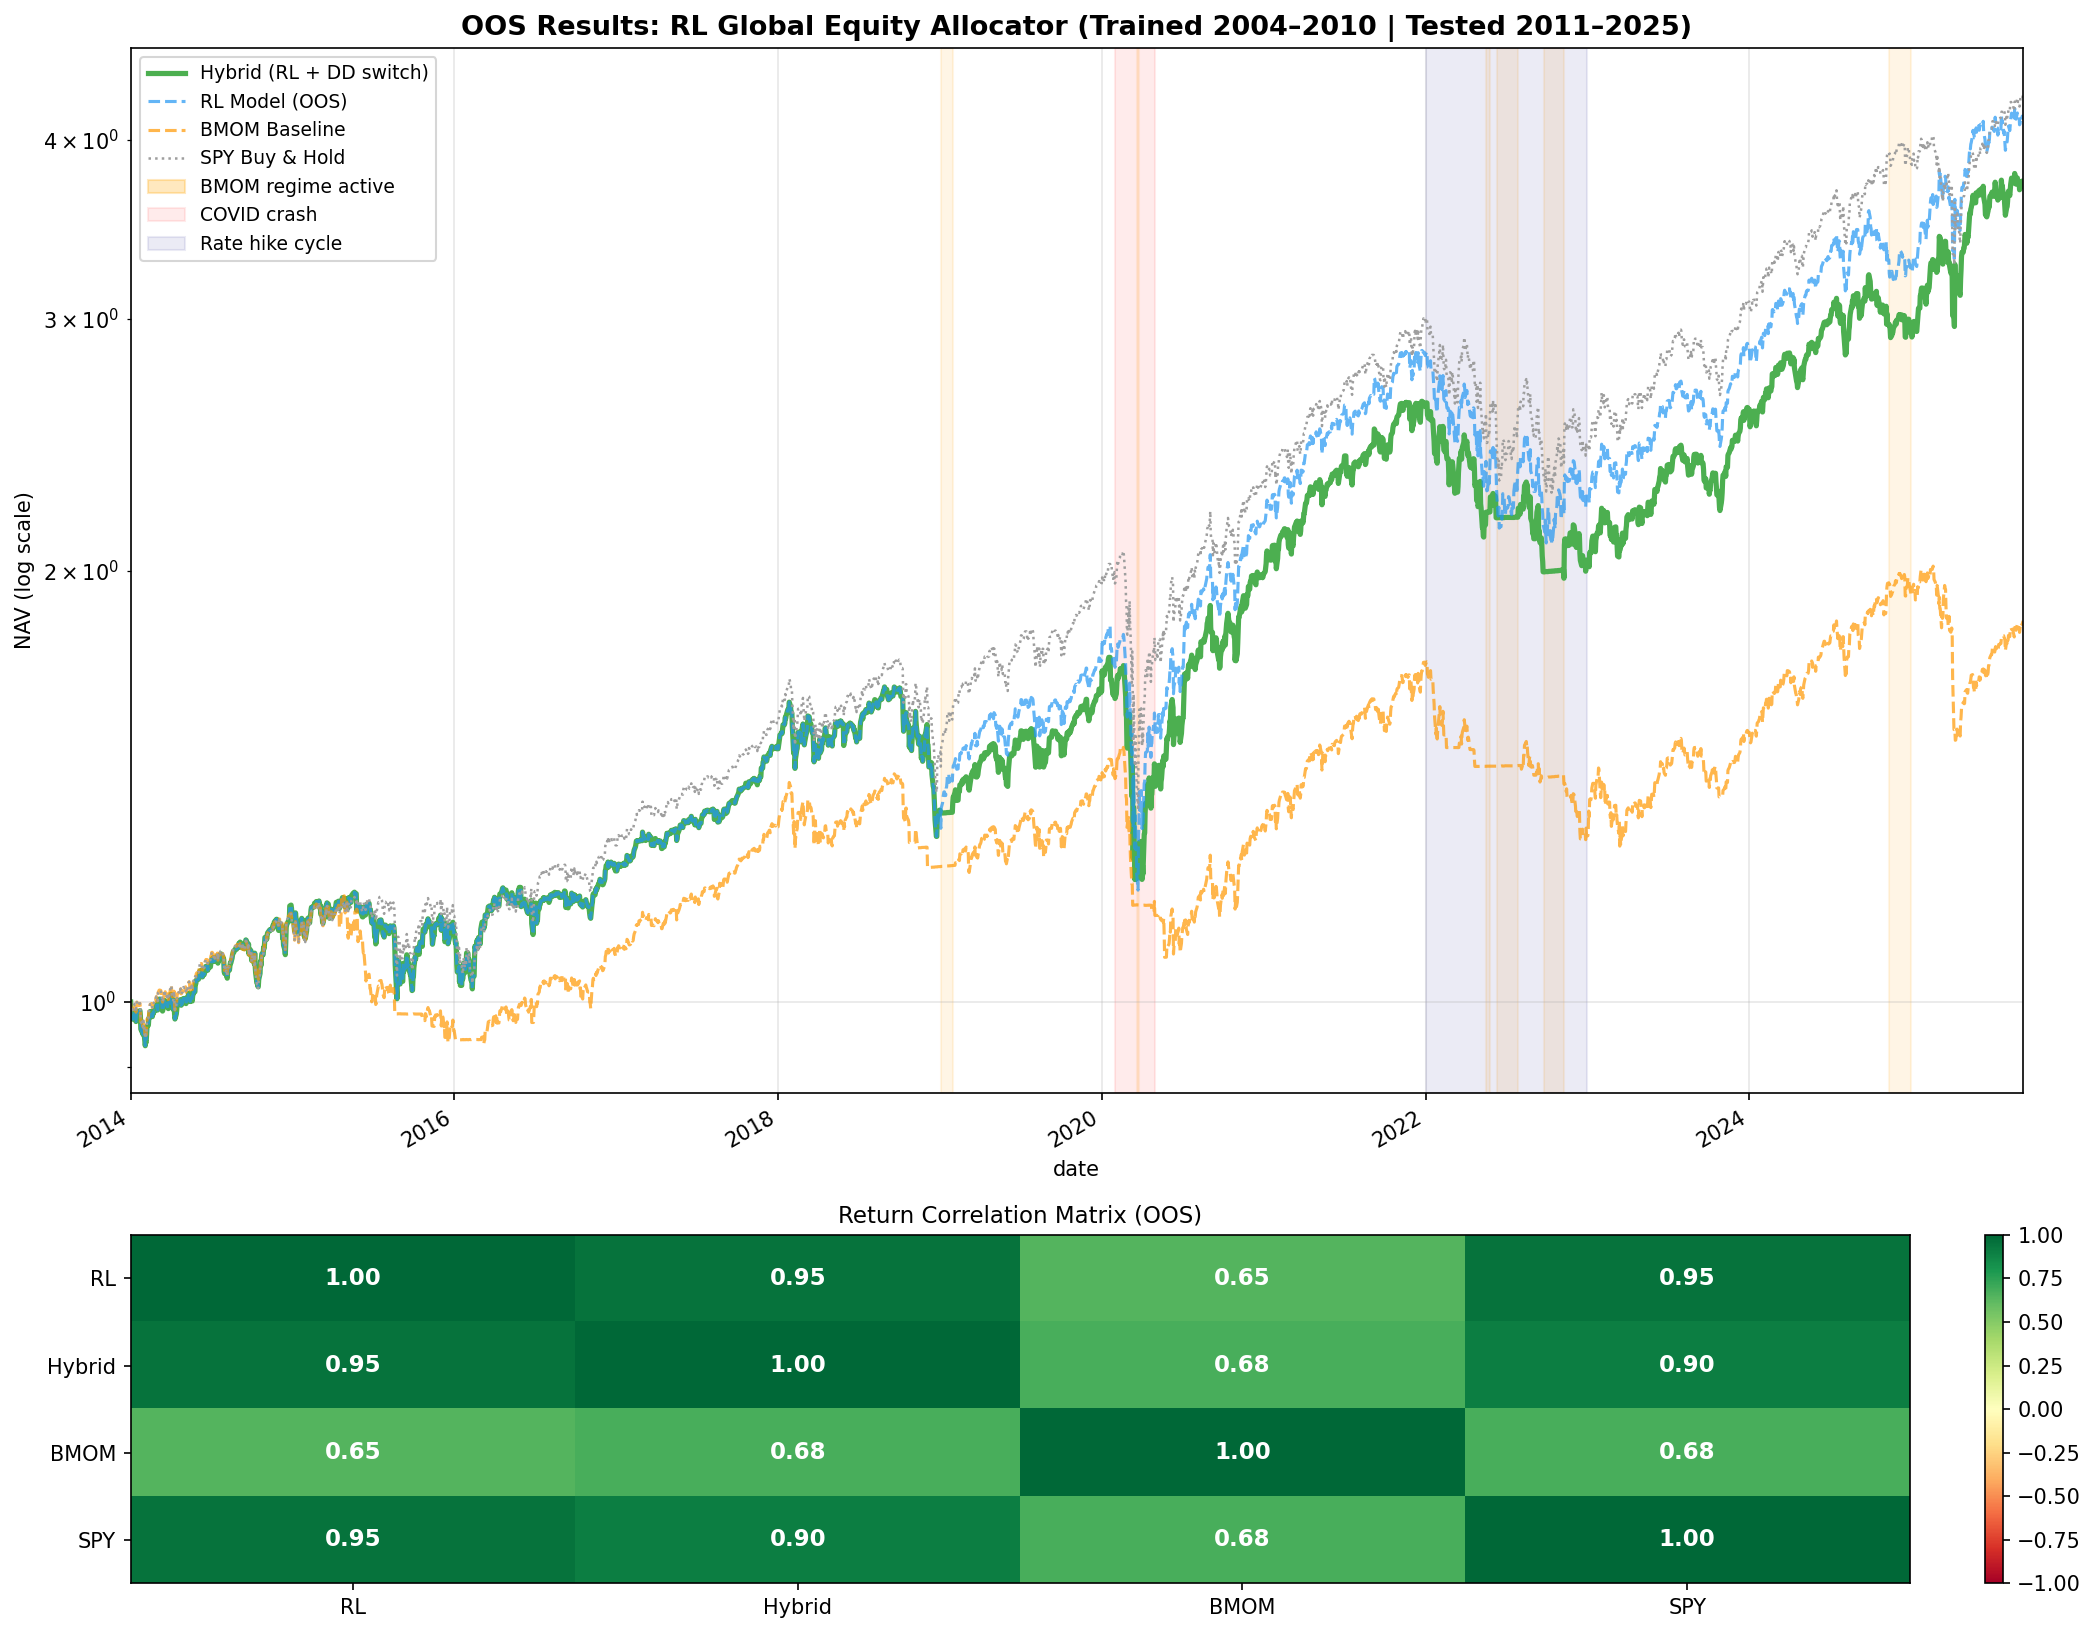
\includegraphics[width=\textwidth]{rl_oos_results.png}
  \caption{OOS equity curves (2014--2025). Hybrid (green), RL standalone (blue dashed), BMOM (orange dashed), SPY (gray). Bottom panel: return correlation heatmap.}
  \label{fig:oos}
\end{figure}

\begin{figure}[H]
  \centering
  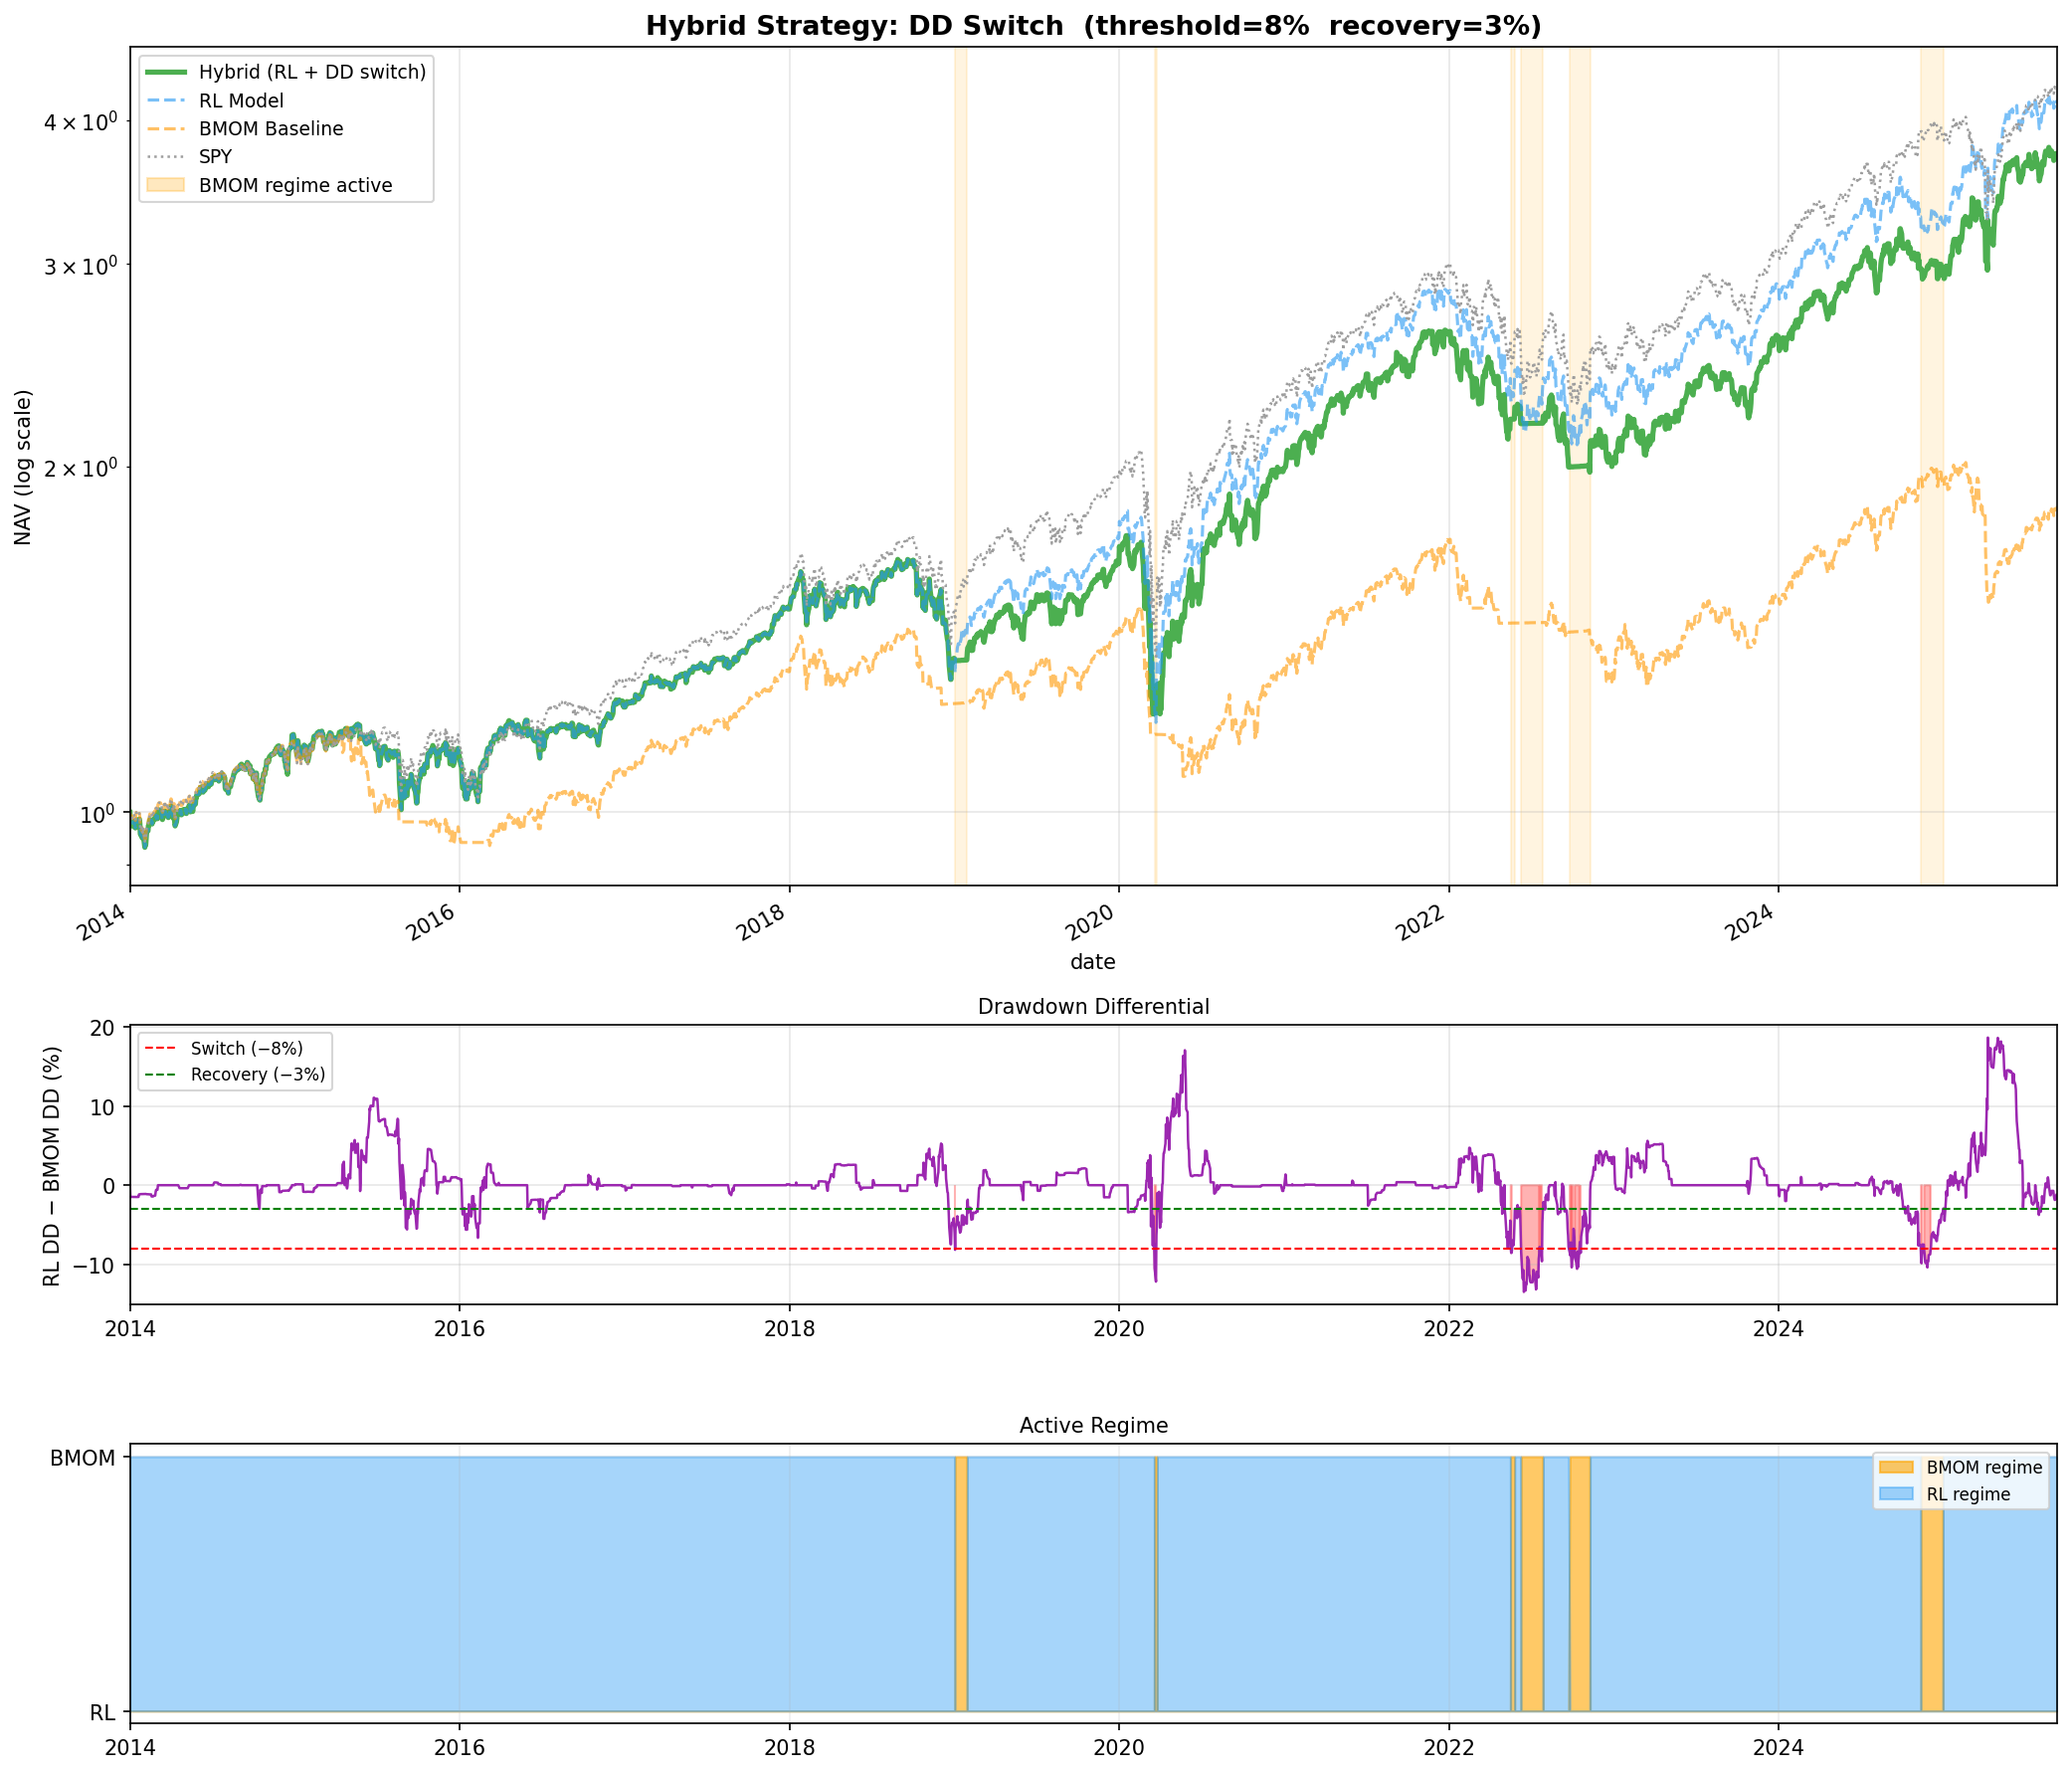
\includegraphics[width=\textwidth]{rl_hybrid_overlay.png}
  \caption{Hybrid overlay mechanics. Top: NAV comparison. Middle: drawdown differential $\Delta(t)$ with $-$8\% trigger and $-$3\% recovery thresholds. Bottom: regime indicator (0 = RL, 1 = BMOM).}
  \label{fig:overlay}
\end{figure}

\begin{figure}[H]
  \centering
  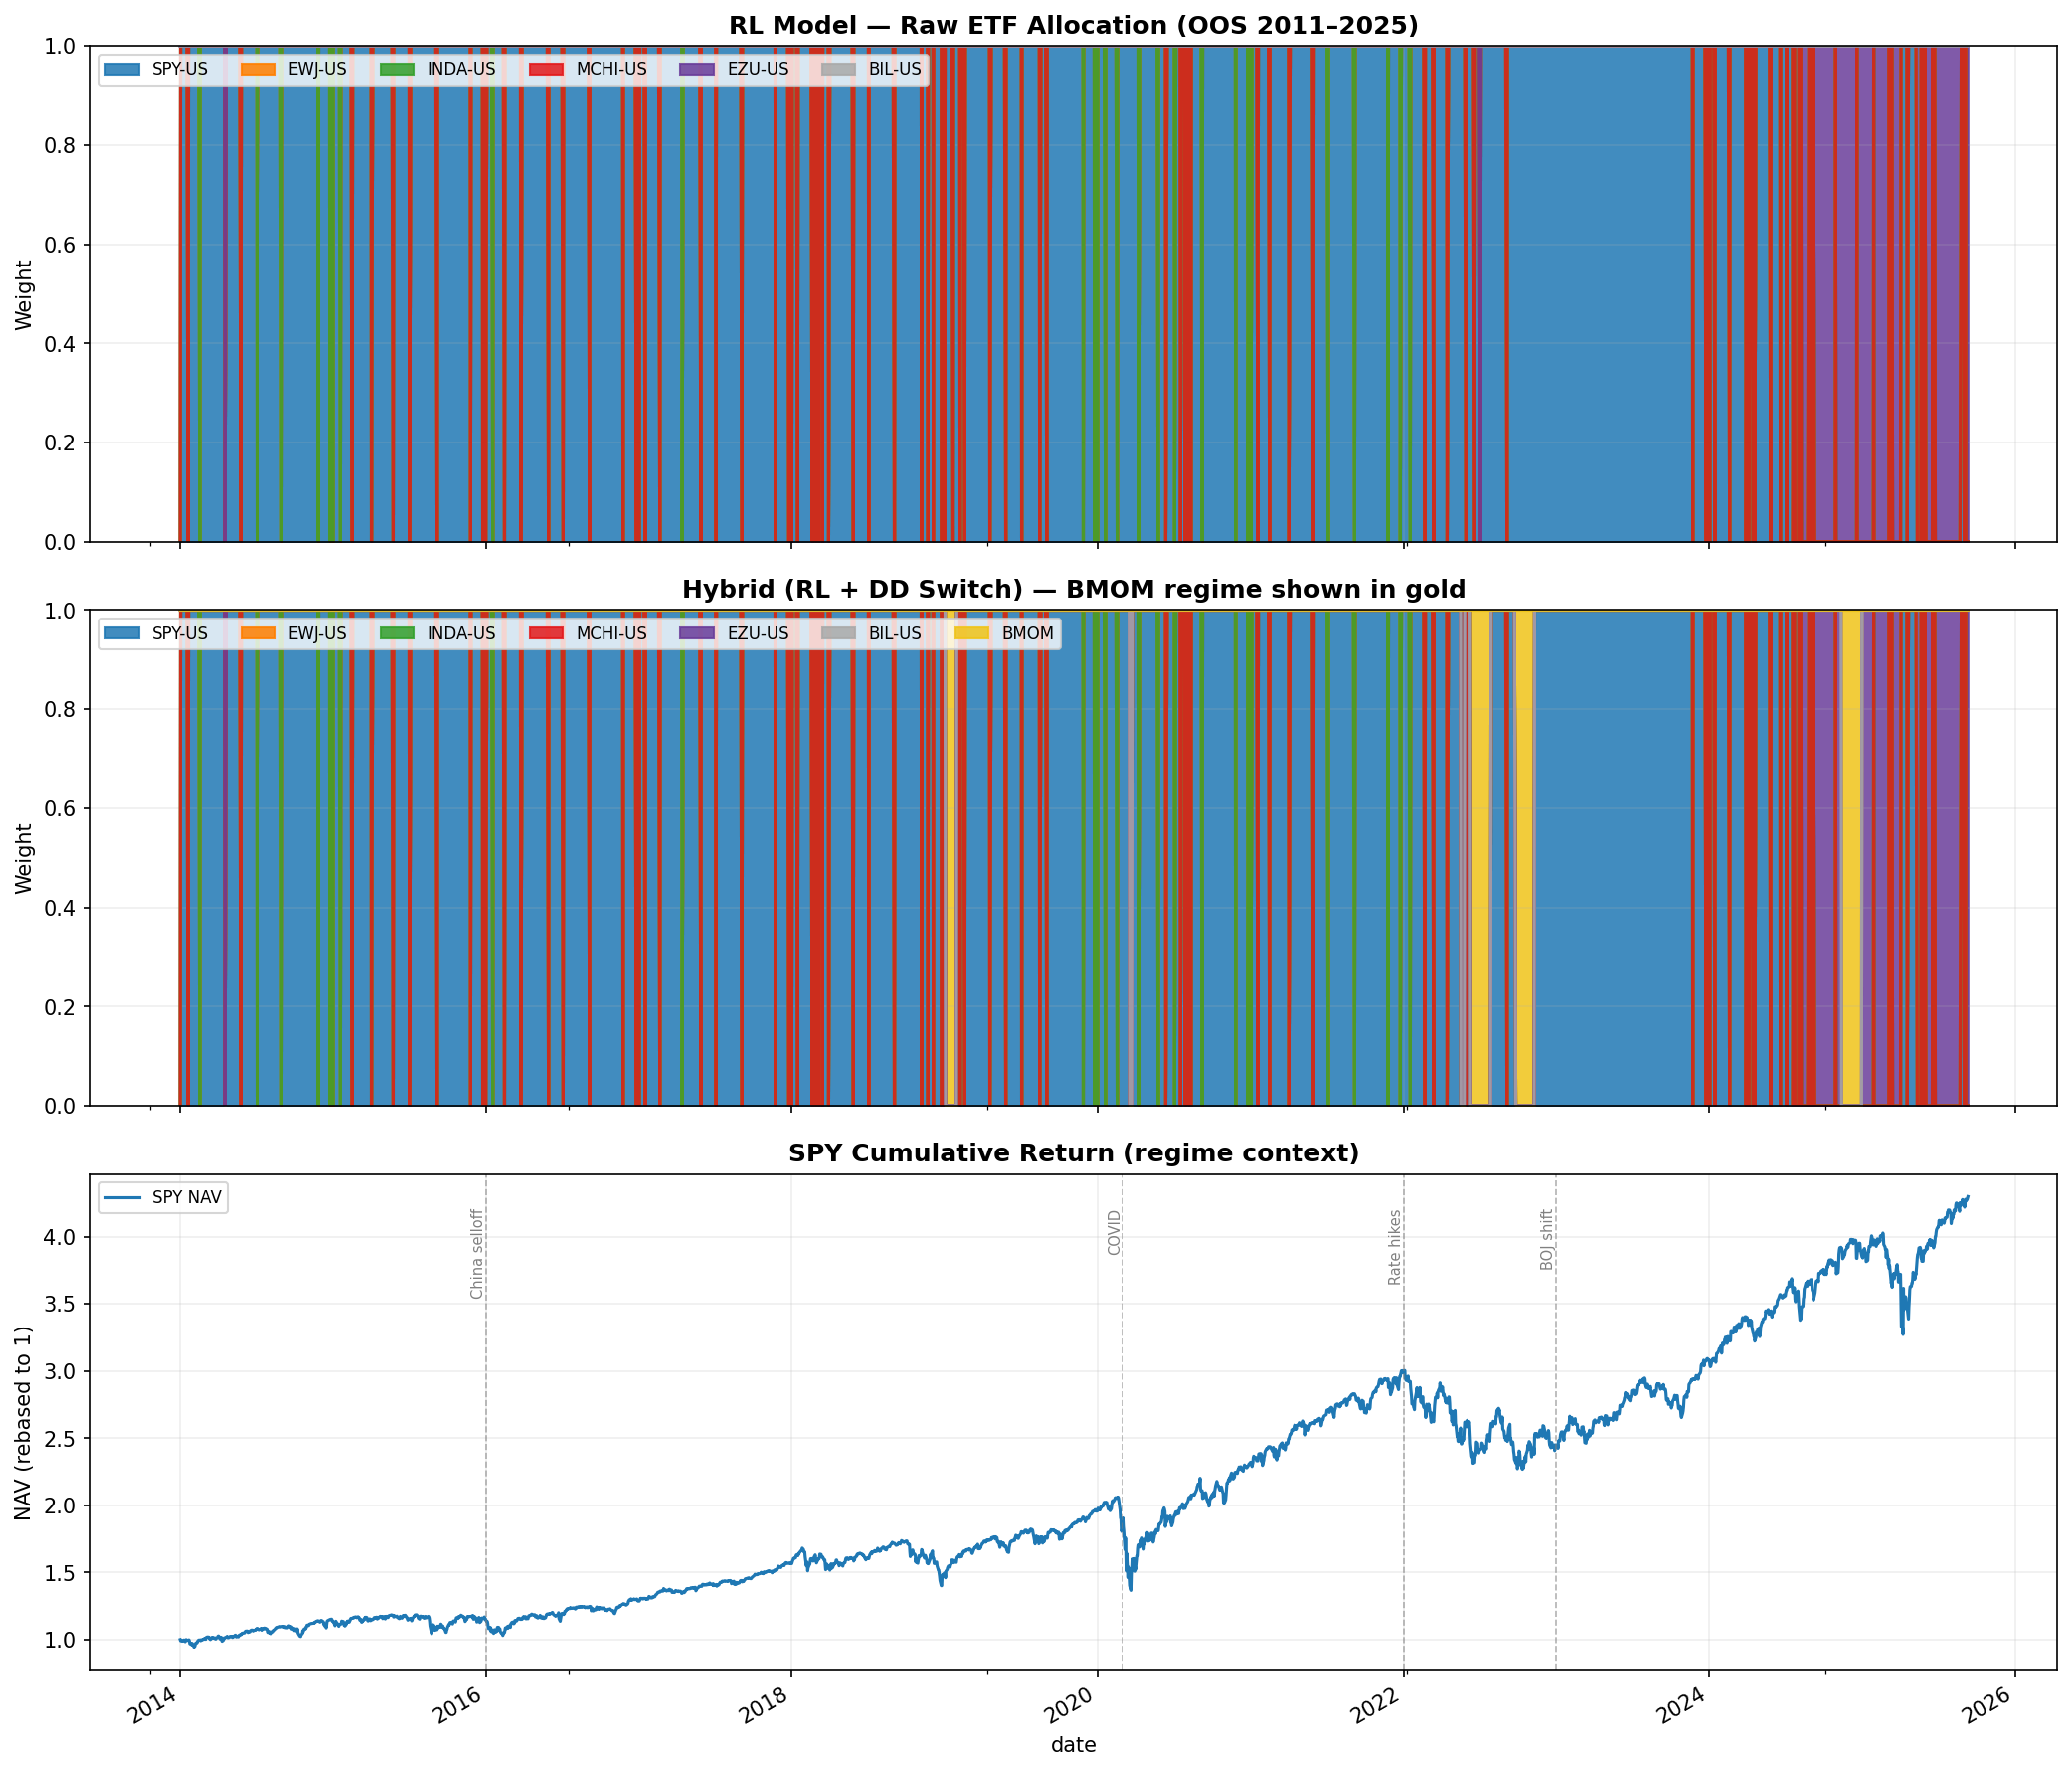
\includegraphics[width=\textwidth]{etf_allocations_over_time.png}
  \caption{ETF allocations over the OOS period. Stacked area shows daily RL model picks; gold shading indicates BMOM regime activation.}
  \label{fig:alloc}
\end{figure}

% ══════════════════════════════════════════════════════════════════════════════
\section{Portfolio Integration}

The hybrid sleeve is evaluated within a mean-variance constrained portfolio alongside 12 AMMA sector models (2020--2025, \$1M initial).

\begin{figure}[H]
  \centering
  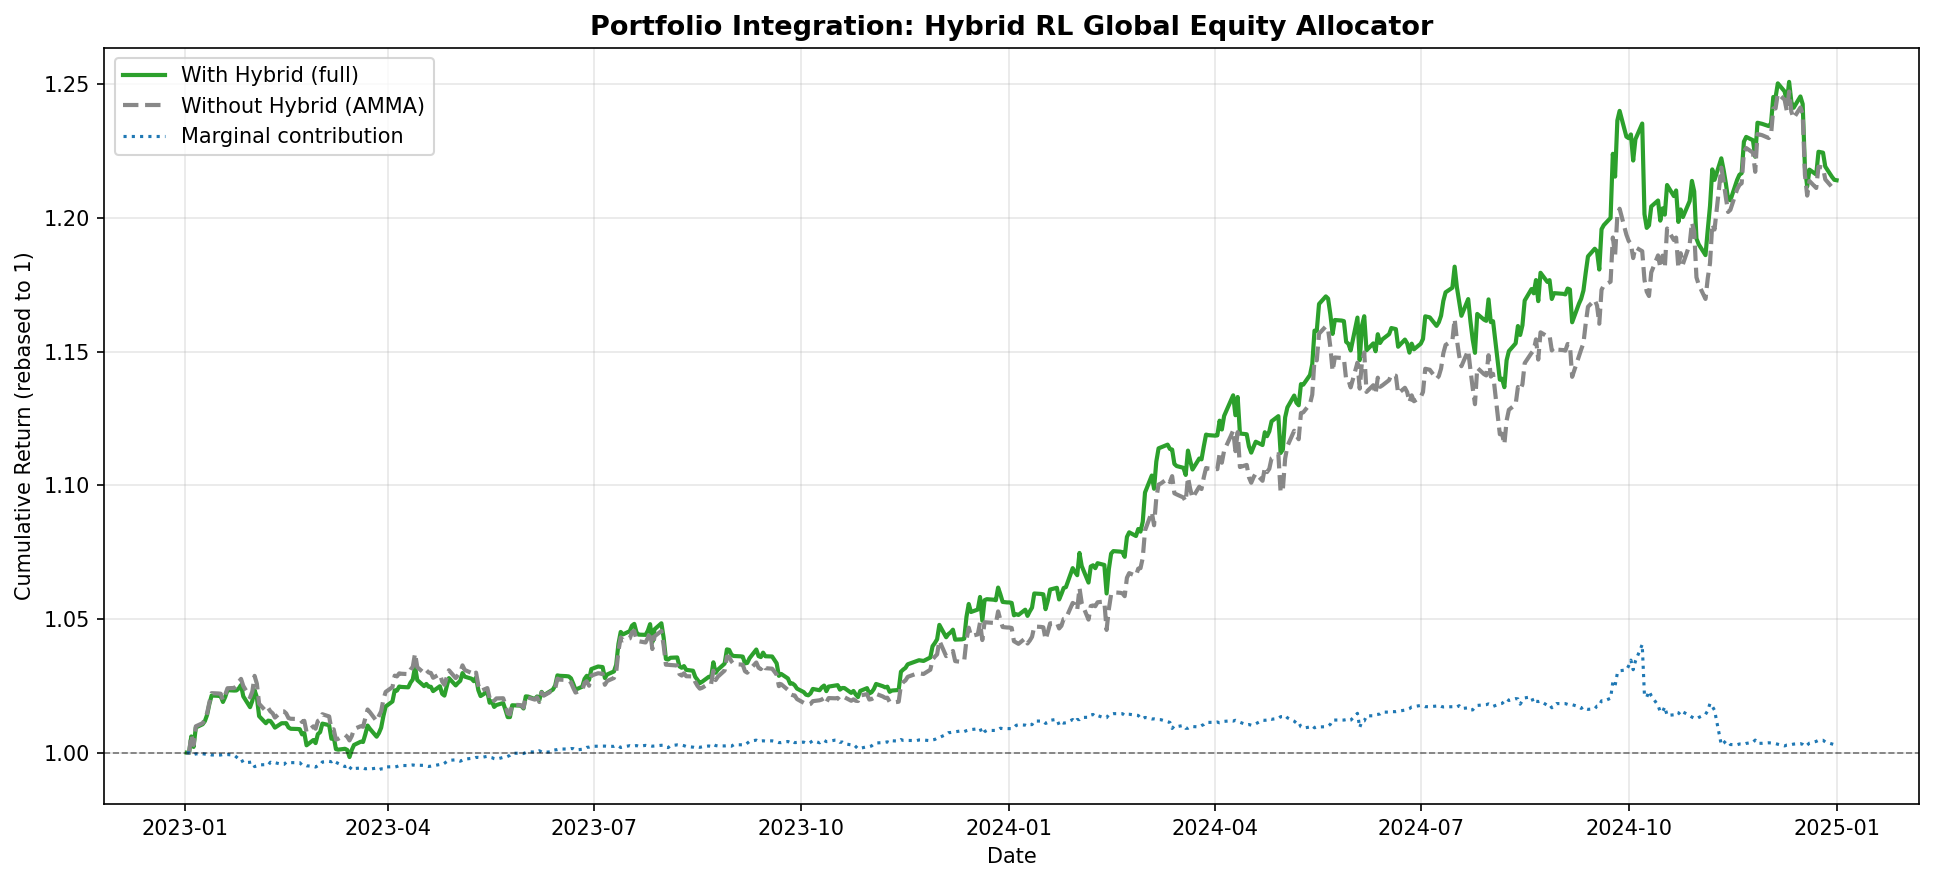
\includegraphics[width=\textwidth]{portfolio_integration.png}
  \caption{Portfolio integration (2020--2025). Green: with hybrid sleeve. Gray dashed: AMMA-only. Blue dotted: marginal contribution ratio.}
  \label{fig:integration}
\end{figure}

The hybrid provides positive marginal contribution across most of the window. Its macro-conditional logic produces returns partially orthogonal to the sector-momentum AMMA models, contributing diversification beyond its standalone volatility.

\textbf{2024 average allocation with hybrid:} SPY 13.1\%, INDA 12.4\%, BIL 11.7\%, SHY 11.0\%, GLD 9.9\%.\\
\textbf{2024 average allocation without hybrid:} BIL 12.9\%, SHY 12.1\%, SPY 11.0\%, GLD 10.1\%.\\
\textbf{Hybrid own allocation (2024):} INDA 59.7\%, SPY 40.3\%.

% ══════════════════════════════════════════════════════════════════════════════
\section{Risk Considerations}

\begin{itemize}[leftmargin=*, itemsep=0.3em]
  \item \textbf{Concentration:} one-hot allocation creates single-asset exposure; the hybrid partially mitigates this.
  \item \textbf{Regime generalisation:} training on 2004--2013 misses post-2010 structural shifts (NIRP, crypto macro, post-COVID fiscal). Strong OOS performance is encouraging but not guaranteed.
  \item \textbf{Seed sensitivity:} Sharpe ranged 0.11--0.73 across seeds. Seed 999 is selected on OOS data, introducing mild seed-selection bias.
  \item \textbf{Data latency:} FRED macro series have release lags of days to weeks; live implementation requires asynchronous handling.
  \item \textbf{Transaction costs:} daily rebalancing assumes close prices with no slippage; emerging-market ETFs (INDA, MCHI) may carry higher impact costs.
\end{itemize}

% ══════════════════════════════════════════════════════════════════════════════
\section{Conclusion}

A PPO agent trained on a compact macro-momentum state space learns durable rotation rules that generalise across 11+ years of unseen data. The standalone model matches SPY returns (13.3\%, Sharpe 0.75) with no post-2013 exposure. The hybrid overlay adds an institutional-grade risk floor (max DD $-$30.0\%, Calmar 0.41) at a cost of 99\,bps. When integrated into a mean-variance portfolio alongside AMMA models, the sleeve delivers incremental risk-adjusted return with positive marginal contribution over 2020--2025.

% ══════════════════════════════════════════════════════════════════════════════
\end{document}
